\documentclass[11pt]{article}

% =====================
% Packages
% =====================
\usepackage[margin=1in]{geometry}
\usepackage[T1]{fontenc}
\usepackage[utf8]{inputenc}
\usepackage{lmodern}
\usepackage{microtype}
\usepackage{graphicx}
\usepackage{amsmath}
\usepackage{xcolor}
\usepackage{booktabs}
\usepackage{enumitem}
\usepackage{titlesec}
\usepackage{fancyhdr}
\usepackage{hyperref}
\usepackage{colortbl}
\usepackage{array}
\usepackage{tabularx}
\usepackage{longtable}
\usepackage{listings}

% =====================
% Colors
% =====================
\definecolor{gamecolor}{HTML}{F5A623}
\definecolor{playercolor}{HTML}{4A90D9}
\definecolor{categorycolor}{HTML}{F8E71C}
\definecolor{platformcolor}{HTML}{7ED321}
\definecolor{submissioncolor}{HTML}{D0021B}
\definecolor{junctioncolor}{HTML}{50E3C2}
\definecolor{headerred}{HTML}{C0392B}
\definecolor{feedbackbg}{HTML}{E8F4FD}
\definecolor{codebg}{HTML}{F5F5F5}
\definecolor{codeframe}{HTML}{CCCCCC}

% =====================
% Listings (SQL)
% =====================
\lstset{
    language=SQL,
    basicstyle=\ttfamily\small,
    backgroundcolor=\color{codebg},
    frame=single,
    rulecolor=\color{codeframe},
    breaklines=true,
    showstringspaces=false,
    keywordstyle=\color{blue}\bfseries,
    commentstyle=\color{gray},
    stringstyle=\color{red!70!black},
    numbers=none,
    xleftmargin=1em,
    framexleftmargin=0.5em
}

% =====================
% Formatting
% =====================
\setlength{\parskip}{0.8em}
\setlength{\parindent}{0pt}

\titleformat{\section}{\Large\bfseries}{\thesection}{1em}{}
\titleformat{\subsection}{\large\bfseries}{\thesubsection}{1em}{}

\pagestyle{fancy}
\fancyhf{}
\rhead{Group 101}
\lhead{CS340 - Project Step 4 Draft}
\rfoot{\thepage}
\renewcommand{\headrulewidth}{0.4pt}

\hypersetup{
    colorlinks=true,
    linkcolor=headerred,
    urlcolor=headerred
}

% =====================
% Custom Commands
% =====================
\newcommand{\entitybox}[2]{%
    \noindent\fcolorbox{black}{#1}{\textbf{\strut\hspace{0.5em}#2\hspace{0.5em}}}%
}

\begin{document}

% =====================
% Title (Header Image)
% =====================
\begin{center}
    
\includegraphics[width=\textwidth]{header.png}
\end{center}

\vspace{0.5em}
\hrulefill

% =====================
% URL (required at top of PDF)
% =====================
\begin{center}
\large\textbf{Live Website:} \url{http://classwork.engr.oregonstate.edu:8742}
\end{center}

\hrulefill

% =====================
% STEP 3 FINAL FEEDBACK
% =====================
\section*{Feedback from Step 3 Final}

Step 3 Final has not yet been graded at the time of this submission. We will incorporate any grading feedback into the next step.

\subsection*{Upgrades for Step 4}

\begin{itemize}[leftmargin=2em]
    \item \textbf{RESET Stored Procedure}: Wrapped the entire DDL (DROP, CREATE, INSERT) into a \texttt{sp\_reset\_database} stored procedure. A ``Reset Database'' button on the home page calls this procedure to restore all tables and sample data.
    \item \textbf{CUD Demo via Stored Procedure}: Created \texttt{sp\_delete\_player\_by\_name} stored procedure in PL.sql. A ``Delete TurboTina'' demo button on the home page calls this SP to demonstrate a CUD operation, which can then be undone by pressing RESET.
    \item \textbf{SELECT on All Entity Pages}: All 6 entity pages (Players, Games, Platforms, RunCategories, RunSubmissions, GamesOnPlatforms) display data from the database using SELECT queries with JOINs for user-friendly FK display.
\end{itemize}

\hrulefill

% =====================
% STEP 3 DRAFT FEEDBACK
% =====================
\section*{Feedback from Step 3 Draft}

We received four peer reviews on our Step 3 Draft submission. The verbatim reviews are included below, followed by our actions.

\textbf{Reviewers:} Kira Stephenson, Adam Fitzpatrick, Trisha Rajesh, Alexa Jauregui.

\subsection*{Verbatim Peer Reviews}

\subsubsection*{Review by Kira Stephenson}
\url{https://edstem.org/us/courses/89768/discussion/7665462?comment=17799317}

\begin{quote}
\textit{Does the UI utilize a SELECT for every table in the schema?}

Yup, the information is clearly presented in the DML file as well (love the comments by the way).

\textit{Does the UI implement an INSERT form for at least one table in the schema?}

There are insert forms for every entity -- Players, Games, Platforms, Run Categories, Run Submissions, and Games on Platforms. Nearly every input field on every single page even has mention of unique input scenarios and whether or not a certain field is optional.

\textit{Does the UI have at least one DELETE for any one entity?}

DELETE is managed by a button that is attached onto anything which has an ID.

\textit{Does the UI have at least one DELETE that will remove things from a M:M relationship?}

Yes. Cascade and constraint operations also appear flawless from what I can tell. Honestly, after reviewing this code I feel ill-equipped with SQL and might need to do some more review; even the JOIN statements are easy to understand.

\textit{Is there at least one UPDATE form in the UI for any one entity?}

Yes. I would maybe consider getting rid of the ability to update rulesets on the Run Categories entity, I only say this because it could allow for people to manipulate the rules for a type of run later on. I think if someone wants to update a ruleset then they should simply make a new run category with a new ruleset rather than being allowed to update previous rules. I know that the down side would be that you can't fix typos or maybe make rules clearer in the future, but that also encourages people to heavily review their rules they initially input rather then just saying ``oh it's fine, I don't need to worry about having good rules since I can just update them later''.

\textit{Is there at least one UPDATE form in the UI to modify an M:M relationship?}

All of your buttons are already functional. WHAT THE HECK?! And yes, the M:M relationships are properly handled because of course they are -- this site is beautiful.

\textit{Do you have any other suggestions for the team to help with their HTML UI?}

Besides the ruleset update allowance I mentioned earlier, I'd say that you might want to include a name of the person who verified a run submission. A run being verified is important, the person who verified the run is even more crucial information to know. At least, that's my opinion.

All of my work is original.
\end{quote}

\subsubsection*{Review by Adam Fitzpatrick}
\url{https://edstem.org/us/courses/89768/discussion/7665462?comment=17821863}

\begin{quote}
\textit{Does the UI utilize a SELECT for every table in the schema?}

The UI does have select Statements for every table in the UI. However when I browsed the site, there were no tables displayed. I'm guessing that this is due to other users, experimenting with the functionality of the UI and not an error in design or implementation.

\textit{Does the UI implement an INSERT form for at least one table in the schema?}

Every table in the UI, with the exception of the intersection table has insert functionality.

\textit{Does the UI have at least one DELETE for any one entity?}

Yes the players table allows for the deletion of individual players.

\textit{Does the UI have at least one DELETE that will remove things from a M:M relationship?}

Yes, and the proper Cascades are defined in the DDL.

\textit{Is there at least one UPDATE form in the UI for any one entity?}

All tables in the UI except for games on platforms have update abilities.

\textit{Is there at least one UPDATE form in the UI to modify an M:M relationship?}

Yes, all of the tables do Already contain functioning update abilities.

\textit{Do you have any other suggestions for the team to help with their HTML UI?}

No real suggestions everything looks to be on track, if not ahead of the game. Possibly populate a larger initial data set. But that isn't entirely necessary.

All work is my own.
\end{quote}

\subsubsection*{Review by Trisha Rajesh}
\url{https://edstem.org/us/courses/89768/discussion/7665462?comment=17824770}

\begin{quote}
\textit{Does the UI utilize a SELECT for every table in the schema?}

Yes there are SELECT queries for every table and each entity has both a general SELECT all and a specific SELECT by ID query.

\textit{Does the UI implement an INSERT form for at least one table in the schema?}

Yes every table in the schema has an INSERT query but I would make sure that for foreign keys, that the dropdowns display meaningful names instead of numeric IDs.

\textit{Does the UI have at least one DELETE for any one entity?}

Yes, each main entity table has a DELETE statement.

\textit{Does the UI have at least one DELETE that will remove things from a M:M relationship?}

Yes the GamesOnPlatforms intersection table handles the many to many relationship between Games and Platforms.

\textit{Is there at least one UPDATE form in the UI for any one entity?}

Yes, update statements exist for all the main entities.

\textit{Is there at least one UPDATE form in the UI to modify an M:M relationship?}

Yes, the table can be updated by deleting the existing relationship and inserting a new one.

\textit{Do you have any other suggestions for the team to help with their HTML UI?}

Dropdown menus for foreign keys should show meaningful values instead of numeric IDs.

This is all my own work.
\end{quote}

\subsubsection*{Review by Alexa Jauregui}
\url{https://edstem.org/us/courses/89768/discussion/7665462?comment=17825970}

\begin{quote}
Hello group 101, your project looks amazing!

\textit{Does the UI utilize a SELECT for every table in the schema?}

Yes, there is a SELECT for each table. Some of the entities don't show any data on the website, but I assume that is because of people experimenting with DELETE.

\textit{Does the UI implement an INSERT form for at least one table in the schema?}

Yes, the UI has an INSERT form section for each entity.

\textit{Does the UI have at least one DELETE for any one entity?}

Yes, there is a DELETE for each entity table. There is a Delete button to the side of each row in a table, which makes it easier for users to delete an item without having to remember which ID they want to delete.

\textit{Does the UI have at least one DELETE that will remove things from a M:M relationship?}

The UI has a DELETE that removes items from M:M relationships. For example, deleting a game will also delete the corresponding rows for games of platform, run submissions, and run categories; this showcases well-implemented Cascade constraints.

\textit{Is there at least one UPDATE form in the UI for any one entity?}

There are UPDATE forms for each entity. When clicking on the update button on the side of the rows, the UPDATE form is populated with the corresponding data.

\textit{Is there at least one UPDATE form in the UI to modify an M:M relationship?}

There is an UPDATE form in the UI to modify M:M relationships. For example, I can choose a different foreign key (like the Run Category) when updating the Run Submissions table. Also, if I update the Run Category, the corresponding tables automatically update the data. Not sure if it's intentional, but the intersection table games on platforms does not offer any update options.

\textit{Do you have any other suggestions for the team to help with their HTML UI?}

Honestly, what you have now looks amazing. I don't have any serious suggestions to make. One improvement could be to add border lines to your tables to make the data more visually appealing, but it's really not necessary.

This is all my original work.
\end{quote}

\subsection*{Actions Based on Step 3 Draft Feedback}

\begin{enumerate}[leftmargin=2em]
    \item \textbf{FK dropdowns showing names instead of IDs} (Trisha Rajesh): Our dropdowns already display meaningful names (e.g., player display names, game titles, platform names) rather than numeric IDs. This was implemented from the start using JOIN queries to populate all dropdown menus. No changes needed.

    \item \textbf{Restrict ruleset updates on Run Categories} (Kira Stephenson): We chose not to implement this restriction. While we understand the concern about rule manipulation, the website is admin-only, so we trust administrators to make responsible edits. Allowing ruleset updates is important for fixing typos and clarifying rules, which is a more common use case than malicious manipulation.

    \item \textbf{Add verifier name to Run Submissions} (Kira Stephenson): We chose not to add a ``verifiedBy'' attribute at this time. Our system is designed for a small nonprofit where the admin team collectively verifies runs. Adding a verifier would require either a new Admins entity or reusing the Players entity, which adds complexity beyond the current scope. The \texttt{verified} boolean and \texttt{verifiedDate} fields are sufficient for the association's needs.

    \item \textbf{Empty tables when browsing} (Adam Fitzpatrick): This was caused by other reviewers experimenting with DELETE functionality during the review period, not a bug. Our DDL.sql can be re-imported to restore sample data at any time.

    \item \textbf{GamesOnPlatforms missing UPDATE} (Alexa Jauregui): This is by design. The intersection table uses an add/remove pattern (INSERT new association, DELETE old association) rather than UPDATE, which is the standard approach for M:N intersection tables. Updating a row in the intersection table would be semantically equivalent to removing one association and creating another.

    \item \textbf{Add border lines to tables} (Alexa Jauregui): Our tables already have subtle styling with alternating row colors and hover effects. We chose not to add additional borders to maintain the clean visual design.

    \item \textbf{Larger initial data set} (Adam Fitzpatrick): We have 5 rows in Players, 4 in Games, 4 in Platforms, 5 in RunCategories, 5 in RunSubmissions, and 7 in GamesOnPlatforms. This meets the 3--5 rows per table requirement and adequately demonstrates all relationship types.
\end{enumerate}

\subsection*{Upgrades to the Step 3 Draft Version}

\begin{itemize}[leftmargin=2em]
    \item \textbf{NULLable Foreign Key -- playerID in RunSubmissions}: Changed the \texttt{playerID} foreign key in RunSubmissions from \texttt{NOT NULL} with \texttt{ON DELETE CASCADE} to \textbf{NULLable} with \texttt{ON DELETE SET NULL}. This means when a Player is deleted, their run submissions are preserved with \texttt{playerID = NULL} (anonymous runs) rather than being cascade-deleted. This satisfies the rubric requirement for at least one NULLable FK relationship and demonstrates a meaningful real-world use case: historical speedrun records should be preserved even if a player leaves the community. The UI displays ``NULL'' for the player field on orphaned submissions, and the Update form allows manually setting a player to NULL. The SELECT query uses a \texttt{LEFT JOIN} on Players (instead of \texttt{INNER JOIN}) so that submissions with \texttt{playerID = NULL} are still displayed.
\end{itemize}

\hrulefill

% =====================
% STEP 2 FEEDBACK
% =====================
\section*{Feedback from Step 2}

Step 2 was a Draft-only submission (no Final version required). We received 100/100 points for turning in the Draft. We received four peer reviews on our Step 2 Draft.

\textbf{Reviewers:} Rebecca Charles, Justin Lee, Ciaran Szwarc, Timothy Birmingham.

\subsection*{Actions Based on Step 2 Feedback}

\begin{enumerate}[leftmargin=2em]
    \item \textbf{Create separate Developers table} (Justin Lee, Ciaran Szwarc, Timothy Birmingham): Chose not to implement. The \texttt{developer} attribute is a simple varchar on Games, not a full entity. Our normalization analysis confirms Games is in 3NF: \texttt{developer} does not functionally determine \texttt{title} or \texttt{releaseYear}. Creating a Developers table for a handful of unique values adds unnecessary complexity with no normalization benefit.

    \item \textbf{Create separate Countries table} (Ciaran Szwarc, Timothy Birmingham): Same reasoning. \texttt{country} is a simple varchar attribute on Players. A lookup table for a small number of values is overengineering for this use case.

    \item \textbf{GamesOnPlatforms: surrogate PK vs composite key} (Rebecca Charles, Ciaran Szwarc): Kept the surrogate \texttt{gameOnPlatformID}. The \texttt{UNIQUE} constraint on \texttt{(gameID, platformID)} prevents duplicates. The surrogate PK simplifies DELETE operations in the UI.

    \item \textbf{Schema line overlap / readability} (All reviewers): Cleaned up the schema and ERD diagrams to reduce line crossings and improve readability.

    \item \textbf{int(11) vs int / year(4) vs year} (Timothy Birmingham): These are phpMyAdmin display artifacts. \texttt{int} and \texttt{int(11)} are identical in MySQL 8.0+. Same for \texttt{year} vs \texttt{year(4)}.

    \item \textbf{videoLink missing from PDF sample data} (Timothy Birmingham): The \texttt{videoLink} column was omitted from the sample data table in the PDF for space but is present in the DDL.sql INSERT statements.
\end{enumerate}

\hrulefill

% =====================
% STEP 1 FEEDBACK
% =====================
\section*{Feedback from Step 1}

We received four peer reviews on our Step 1 Draft submission. Below is a summary of the feedback and actions taken.

\textbf{Reviewers:} Kain Sherman, Olivia Choi, Bryant Aragon, Lucas Feldsien.

\subsection*{Actions Based on Step 1 Feedback}

Based on the peer reviews, we made the following corrections:

\begin{enumerate}[leftmargin=2em]
    \item \textbf{Naming Consistency -- Singular to Plural} (Kain Sherman): Changed all entity names from singular to plural (Game $\rightarrow$ Games, Player $\rightarrow$ Players, RunCategory $\rightarrow$ RunCategories, Platform $\rightarrow$ Platforms, RunSubmission $\rightarrow$ RunSubmissions) to follow the rubric's suggested convention.

    \item \textbf{Intersection Table Naming Inconsistency} (Kain Sherman): Fixed the inconsistency between the ERD and Relationship Summary table. The table previously mentioned ``GamePlatforms'' while the ERD showed ``GameOnPlatform.'' We standardized to ``GamesOnPlatforms'' (plural, matching our other entity naming convention) across both the ERD and all documentation.

    \item \textbf{Game-RunCategory Relationship Wording Confusion} (Kain Sherman, Lucas Feldsien): Both reviewers identified that the relationship description was contradictory -- the Game section implied one RunCategory could be associated with many Games, while the RunCategory section stated it could only belong to one Game. We corrected this by clarifying that the relationship is 1:M from Games to RunCategories: one Game can have multiple RunCategories, but each RunCategory belongs to exactly one Game. The gameID FK in RunCategories enforces this constraint.

    \item \textbf{Numerical Scope -- Annual Run Estimates} (Kain Sherman, Olivia Choi): Kain suggested more concrete numbers to scope the system, and Olivia specifically recommended estimating annual run submissions. We added the calculation: with 25--100 players per competition and 1--30 runs per player per year, the system is expected to handle approximately 750--3,000 run submissions annually.

    \item \textbf{Entity Highlighting in Overview} (Kain Sherman): Added colored highlighting to entity names in the Overview section so they can be quickly mapped to the Database Outline, improving readability as suggested.

    \item \textbf{Verification Date Attribute} (Olivia Choi): Added \texttt{verifiedDate: date} attribute to RunSubmissions to track when a run was verified by an admin, supporting admin workflows and record-keeping as suggested.

    \item \textbf{User Roles Clarification} (Olivia Choi): Clarified in the Overview that the website will be ``editable by admins, and viewable by players,'' explicitly stating who will use the site and their primary actions as suggested.

    \item \textbf{Run Category Edge Cases} (Olivia Choi): Olivia asked whether every run submission must always belong to exactly one category. We confirm this is by design: each RunSubmission has a NOT NULL FK to RunCategories, enforcing that every run belongs to exactly one category. This matches standard speedrunning practice where runs are submitted to specific categories with distinct rulesets (e.g., a ``100\%'' run cannot simultaneously be an ``Any\%'' run).
\end{enumerate}

\subsection*{Additional Design Changes for Step 2}

\begin{itemize}[leftmargin=2em]
    \item \textbf{Normalization Verified}: Applied the normalization process to all tables \textit{(details in the Normalization section below)}. All tables satisfy 3NF.
    \item \textbf{CASCADE Constraints}: Added ON DELETE CASCADE and ON UPDATE CASCADE to all foreign key constraints, as recommended by the course materials. \textit{Note: For Step 3 Final, playerID in RunSubmissions was changed to ON DELETE SET NULL -- see ``Upgrades to the Step 3 Draft Version'' above.}
    \item \textbf{Schema Diagram}: Created based on DDL implementation, generated using phpMyAdmin Designer.
    \item \textbf{Example Data}: Added 3--5 rows of sample data per table that demonstrate all relationship types in action.
\end{itemize}

\hrulefill

% =====================
% b) OVERVIEW AND DATABASE OUTLINE (Updated)
% =====================
\section*{b) Project Overview and Database Outline -- Updated Version}

\subsection*{Overview}

\textit{The following overview is a fictional scenario we are using as a framework for our project.}

\textbf{Northern Oregon Speedrunners Association} is a nonprofit organization that runs various video game speedrunning events in local communities in Northern Oregon. They would like to have a website where they can store the various speedrun submissions from their competitions, which typically consist of 25--100 players, depending on the competition. The amount of runs submitted per year will vary drastically, depending on activity in the local speedrunning community, but on average most players will submit 1--30 runs per year. Based on these figures, the system is expected to handle approximately 750--3,000 \textbf{run submissions} annually.

Due to the limited needs of this system, they don't need a way to categorize the runs by the event they are a part of, and storing them by date is enough information for them to infer the event they are from. This then allows users to submit runs to be verified that they may complete from home by sending the info about their run to an administrator of the association.

The association only wants \colorbox{submissioncolor!30}{\textbf{run submissions}} to be able to be submitted by admin board members of the association. They would like to be able to see the name of the \colorbox{playercolor!30}{\textbf{players}}, the runs they have successfully completed, what \colorbox{gamecolor!30}{\textbf{game}} they speedran, what \colorbox{categorycolor!30}{\textbf{run categories}} these runs are in, and what \colorbox{platformcolor!30}{\textbf{platform}} they were on when they completed the run. This information will serve as a record for all local speedrunners in the area to show off their previous times, and gives \textbf{Northern Oregon Speedrunners Association} a record to determine local speedrunning records. This website will be editable by admins, and viewable by players.

\textit{Extra Note: To accommodate for players who may have moved to a different part of the world, the player entity will contain a country.}

\subsection*{Database Outline}

% --- Players ---
\subsubsection*{\entitybox{playercolor}{Players}}
\textit{Description: A speedrunner participant (via a displayName) that can speedrun various games.}

\begin{itemize}[leftmargin=1.5em]
    \item \textbf{playerID}: int, auto\_increment, unique, not NULL, PK
    \item \textbf{displayName}: varchar(100), not NULL, unique -- The player's username/unique handle
    \item \textbf{country}: varchar(100) -- The player's country of residence
\end{itemize}

\textbf{Relationship(s):}
\begin{itemize}[leftmargin=2.5em]
    \item 1:M with RunSubmissions with playerID as a NULLable FK in RunSubmissions (one Player can have many RunSubmissions; ON DELETE SET NULL)
\end{itemize}

\hrulefill

% --- Games ---
\subsubsection*{\entitybox{gamecolor}{Games}}
\textit{Description: A video game that is able to be speedrun.}

\begin{itemize}[leftmargin=1.5em]
    \item \textbf{gameID}: int, auto\_increment, unique, not NULL, PK
    \item \textbf{title}: varchar(255), not NULL -- The name of the video game
    \item \textbf{releaseYear}: YEAR -- Year the game was released
    \item \textbf{developer}: varchar(255) -- The company that developed the game
\end{itemize}

\textbf{Relationship(s):}
\begin{itemize}[leftmargin=2.5em]
    \item 1:M with RunSubmissions with gameID as a FK in RunSubmissions (one Game can have many RunSubmissions)
    \item 1:M with RunCategories with gameID as a FK in RunCategories (one Game can have multiple RunCategories)
    \item M:N with Platforms via \textit{GamesOnPlatforms} intersection table with both gameID and platformID as FKs (one Game can be on many Platforms; one Platform can have many Games)
\end{itemize}

\hrulefill

% --- RunCategories ---
\subsubsection*{\entitybox{categorycolor}{RunCategories}}
\textit{Description: A speedrun submission type which different games provide.}

\begin{itemize}[leftmargin=1.5em]
    \item \textbf{runCategoryID}: int, auto\_increment, unique, not NULL, PK
    \item \textbf{name}: varchar(100), not NULL -- The category name (e.g., ``Any\%'', ``Glitchless'', ``100\%'')
    \item \textbf{ruleset}: text -- Description of rules for this category
    \item \textbf{gameID}: int, not NULL, FK -- References Games.gameID
\end{itemize}

\textbf{Relationship(s):}
\begin{itemize}[leftmargin=2.5em]
    \item 1:M with RunSubmissions with runCategoryID as a FK in RunSubmissions (one RunCategory can have many RunSubmissions)
    \item M:1 with Games with gameID as a FK in this RunCategories table (each RunCategory belongs to one and only one Game)
\end{itemize}

\hrulefill

% --- Platforms ---
\subsubsection*{\entitybox{platformcolor}{Platforms}}
\textit{Description: The hardware or environment a game can be played on.}

\begin{itemize}[leftmargin=1.5em]
    \item \textbf{platformID}: int, auto\_increment, unique, not NULL, PK
    \item \textbf{name}: varchar(100), not NULL, unique -- The platform name (e.g., ``PC'', ``Nintendo Switch'', ``PlayStation 5'')
\end{itemize}

\textbf{Relationship(s):}
\begin{itemize}[leftmargin=2.5em]
    \item 1:M with RunSubmissions with platformID as a FK in RunSubmissions (one Platform can have many RunSubmissions)
    \item M:N with Games via \textit{GamesOnPlatforms} intersection table with both platformID and gameID as FKs (one Platform can have many Games; one Game can be on many Platforms)
\end{itemize}

\hrulefill

% --- RunSubmissions ---
\subsubsection*{\entitybox{submissioncolor!80}{RunSubmissions}}
\textit{Description: A specific speedrun record that has all the information about that speedrun attempt.}

\begin{itemize}[leftmargin=1.5em]
    \item \textbf{runSubmissionID}: int, auto\_increment, unique, not NULL, PK
    \item \textbf{runTime}: time(3), not NULL -- The duration of the speedrun (HH:MM:SS.mmm)
    \item \textbf{submissionDate}: date, not NULL -- The date the run was submitted
    \item \textbf{verified}: boolean, default FALSE -- Whether the run has been verified by an admin
    \item \textbf{verifiedDate}: date -- The date the run was verified (NULL if not yet verified)
    \item \textbf{playerID}: int, FK -- References Players.playerID (NULLable; ON DELETE SET NULL)
    \item \textbf{gameID}: int, not NULL, FK -- References Games.gameID
    \item \textbf{platformID}: int, not NULL, FK -- References Platforms.platformID
    \item \textbf{runCategoryID}: int, not NULL, FK -- References RunCategories.runCategoryID
    \item \textbf{videoLink}: varchar(2048) -- URL to video proof of the run
\end{itemize}

\textbf{Relationship(s):}
\begin{itemize}[leftmargin=2.5em]
    \item M:1 with Players with playerID as a NULLable FK in this RunSubmissions table (many RunSubmissions belong to one Player; ON DELETE SET NULL preserves runs when a Player is deleted)
    \item M:1 with Games with gameID as a FK in this RunSubmissions table (many RunSubmissions belong to one Game)
    \item M:1 with Platforms with platformID as a FK in this RunSubmissions table (many RunSubmissions were played on one Platform)
    \item M:1 with RunCategories with runCategoryID as a FK in this RunSubmissions table (many RunSubmissions are in one RunCategory)
\end{itemize}

\hrulefill

% --- GamesOnPlatforms ---
\subsubsection*{\entitybox{junctioncolor}{GamesOnPlatforms} \normalfont\textit{(Intersection Table)}}
\textit{Description: Tracks which games are available on which platforms (M:N relationship).}

\begin{itemize}[leftmargin=1.5em]
    \item \textbf{gameOnPlatformID}: int, auto\_increment, unique, not NULL, PK
    \item \textbf{gameID}: int, not NULL, FK -- References Games.gameID
    \item \textbf{platformID}: int, not NULL, FK -- References Platforms.platformID
\end{itemize}

\textbf{Constraint:} Unique combination of (gameID, platformID)

% =====================
% Relationship Summary
% =====================
\subsection*{Relationship Summary}

\begin{center}
\begin{tabular}{lll}
\toprule
\textbf{Relationship} & \textbf{Type} & \textbf{Implementation} \\
\midrule
Players $\rightarrow$ RunSubmissions & 1:M & playerID NULLable FK in RunSubmissions (SET NULL) \\
Games $\rightarrow$ RunSubmissions & 1:M & gameID FK in RunSubmissions \\
Platforms $\rightarrow$ RunSubmissions & 1:M & platformID FK in RunSubmissions \\
RunCategories $\rightarrow$ RunSubmissions & 1:M & runCategoryID FK in RunSubmissions \\
Games $\leftrightarrow$ Platforms & M:N & GamesOnPlatforms intersection table \\
Games $\rightarrow$ RunCategories & 1:M & gameID FK in RunCategories \\
\bottomrule
\end{tabular}
\end{center}

\textbf{Total: 6 relationships (including 1 M:N) across 6 tables}

\hrulefill

% =====================
% c) ERD
% =====================
\section*{c) Entity-Relationship Diagram}

\textit{Demonstrates a visual representation of the relationships between the entities listed above. Only primary keys are shown in the ERD; full attributes are listed in the Database Outline above and the Schema Diagram below.}

\begin{center}
    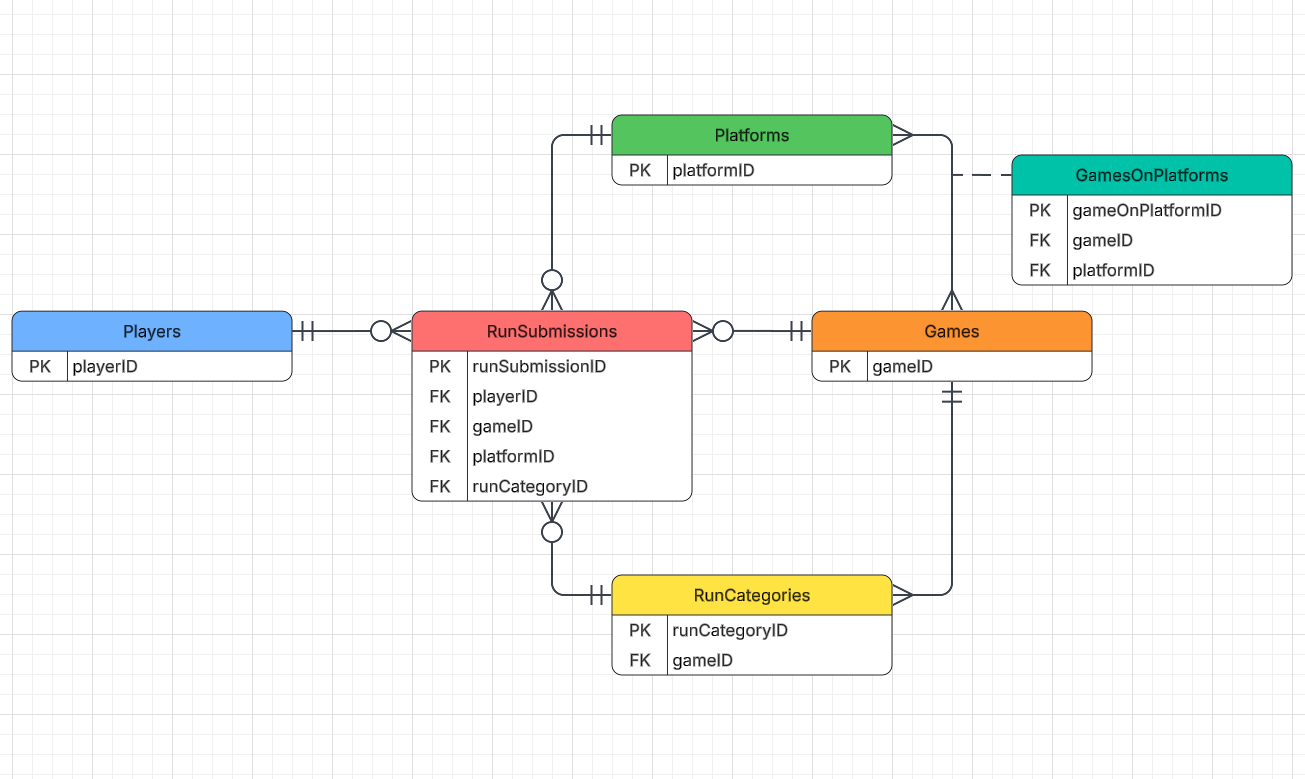
\includegraphics[width=\textwidth]{erd.png}
\end{center}

\textit{Note: The ERD matches the Database Outline and Schema Diagram. All entity names are plural, the intersection table is named GamesOnPlatforms, and the verifiedDate attribute has been added to RunSubmissions.}

\hrulefill

% =====================
% NORMALIZATION ANALYSIS (new for Step 2)
% =====================
\section*{Normalization Analysis}

We applied the normalization process that we learned about in the Exploration -- Normalization Steps. We started by examining a hypothetical sample report (similar to the construction company example from the exploration) and checked for redundancies and anomalies.

\subsection*{Hypothetical Denormalized Report}

Consider a report of various speedruns that an administrator would want to add to the database, listing all run submissions based on the following criteria:

\begin{center}
\footnotesize
\begin{tabular}{llllllll}
\toprule
\textbf{Player} & \textbf{Country} & \textbf{Game} & \textbf{Developer} & \textbf{Category} & \textbf{Platform} & \textbf{RunTime} & \textbf{Verified} \\
\midrule
SpeedDemon42 & US & Mario 64 & Nintendo & Any\% & N64 & 15:35 & Yes \\
SpeedDemon42 & US & Mario 64 & Nintendo & 16 Star & N64 & 49:12 & Yes \\
PixelRunner & CA & Zelda: OoT & Nintendo & Any\% & Switch & 18:22 & No \\
GlitchHunter & US & Celeste & MaddyMakes & Any\% & PC & 32:45 & Yes \\
NightOwlPlays & JP & Portal & Valve & Inbounds & PC & 14:08 & No \\
\bottomrule
\end{tabular}
\end{center}

\subsection*{Redundancy and Anomaly Analysis}

If all data were stored in a single flat table:

\begin{itemize}[leftmargin=2em]
    \item \textbf{Redundant Data}: ``SpeedDemon42'' and ``US'' are repeated for each run by that player. ``Nintendo'' is repeated for each game developed by Nintendo. ``Super Mario 64'' is repeated for each run of that game.
    \item \textbf{Insert Anomaly}: To add a new game, we would need to create a dummy run submission. To add a new player, we would need a dummy run.
    \item \textbf{Update Anomaly}: Changing a player's country would require updating every row with that player. Changing a game's developer would require updating every run for that game.
    \item \textbf{Delete Anomaly}: Deleting the only run for a game would lose all information about that game. Deleting the only run for a player would lose that player's information.
\end{itemize}

\subsection*{1NF Verification}

All tables in the final Schema are in 1NF:
\begin{itemize}[leftmargin=2em]
    \item Every table has a defined primary key (no repeating groups).
    \item All attributes contain atomic values (single value per cell, no lists or sets).
    \item No table has repeating groups -- each row is uniquely identifiable by its PK.
\end{itemize}

\subsection*{2NF Verification}

All tables in the final Schema are in 2NF:
\begin{itemize}[leftmargin=2em]
    \item No table has a composite primary key with partial dependencies. Players, Games, Platforms, RunCategories, and RunSubmissions all use single-column auto-increment primary keys, so partial dependency is impossible.
    \item The GamesOnPlatforms table contains no non-key attributes beyond the two foreign keys, so there are no partial dependencies.
\end{itemize}

\subsection*{3NF Verification}

All tables in the final Schema are in 3NF:
\begin{itemize}[leftmargin=2em]
    \item \textbf{Players}: \texttt{playerID} $\rightarrow$ \texttt{displayName}, \texttt{country}. No transitive dependency (country does not determine any other non-key attribute).
    \item \textbf{Games}: \texttt{gameID} $\rightarrow$ \texttt{title}, \texttt{releaseYear}, \texttt{developer}. No transitive dependency (developer is an independent non-key attribute and does not functionally determine \texttt{title} or \texttt{releaseYear}; multiple games can share the same developer while having different titles and release years, so there is no transitive dependency among non-key attributes).
    \item \textbf{Platforms}: \texttt{platformID} $\rightarrow$ \texttt{name}. Only one non-key attribute; no transitive dependency possible.
    \item \textbf{RunCategories}: \texttt{runCategoryID} $\rightarrow$ \texttt{name}, \texttt{ruleset}, \texttt{gameID}. The gameID is a FK, not a transitive determinant. The name and ruleset are specific to the category, not determined by gameID alone (one game has multiple categories with different names and rulesets).
    \item \textbf{RunSubmissions}: \texttt{runSubmissionID} $\rightarrow$ all other attributes. All non-key attributes (runTime, submissionDate, verified, verifiedDate, videoLink) are facts about the specific run submission, not about any other non-key attribute. The FKs (playerID, gameID, platformID, runCategoryID) reference other tables -- they do not transitively determine each other.
    \item \textbf{GamesOnPlatforms}: Contains only the surrogate PK and two FKs. No non-key attributes to create transitive dependencies.
\end{itemize}

\textbf{Conclusion}: All six tables satisfy 3NF. No denormalization decisions were necessary, as the schema was already properly decomposed from the initial design in Step 1.

\hrulefill

% =====================
% d) SCHEMA DIAGRAM
% =====================
\section*{d) Schema Diagram}

The schema diagram below was generated from phpMyAdmin Designer after importing the DDL into the CS340 class database on the ENGR server. It shows all tables, their columns, primary keys, and foreign key relationships.

\begin{center}
    
\includegraphics[width=\textwidth]{schema-diagram.png}
\end{center}

\textit{Note: This schema matches the Database Outline and ERD exactly. All foreign keys use ON DELETE CASCADE and ON UPDATE CASCADE constraints, except for \texttt{playerID} in RunSubmissions which uses ON DELETE SET NULL (NULLable FK relationship).}

The following tables provide a detailed textual reference for each table's attributes and constraints:

\vspace{1em}

\begin{center}
\small
\renewcommand{\arraystretch}{1.2}

% -- Players --
\begin{tabular}{|l|l|l|}
\hline
\rowcolor{playercolor!30}
\multicolumn{3}{|c|}{\textbf{Players}} \\
\hline
\textbf{Attribute} & \textbf{Type} & \textbf{Constraints} \\
\hline
\underline{playerID} & int & PK, auto\_increment, NOT NULL \\
displayName & varchar(100) & NOT NULL, UNIQUE \\
country & varchar(100) & \\
\hline
\end{tabular}

\vspace{1.5em}

% -- Games --
\begin{tabular}{|l|l|l|}
\hline
\rowcolor{gamecolor!30}
\multicolumn{3}{|c|}{\textbf{Games}} \\
\hline
\textbf{Attribute} & \textbf{Type} & \textbf{Constraints} \\
\hline
\underline{gameID} & int & PK, auto\_increment, NOT NULL \\
title & varchar(255) & NOT NULL \\
releaseYear & YEAR & \\
developer & varchar(255) & \\
\hline
\end{tabular}

\vspace{1.5em}

% -- Platforms --
\begin{tabular}{|l|l|l|}
\hline
\rowcolor{platformcolor!30}
\multicolumn{3}{|c|}{\textbf{Platforms}} \\
\hline
\textbf{Attribute} & \textbf{Type} & \textbf{Constraints} \\
\hline
\underline{platformID} & int & PK, auto\_increment, NOT NULL \\
name & varchar(100) & NOT NULL, UNIQUE \\
\hline
\end{tabular}

\vspace{1.5em}

% -- RunCategories --
\begin{tabular}{|l|l|l|}
\hline
\rowcolor{categorycolor!30}
\multicolumn{3}{|c|}{\textbf{RunCategories}} \\
\hline
\textbf{Attribute} & \textbf{Type} & \textbf{Constraints} \\
\hline
\underline{runCategoryID} & int & PK, auto\_increment, NOT NULL \\
name & varchar(100) & NOT NULL \\
ruleset & text & \\
gameID & int & FK $\rightarrow$ Games.gameID, NOT NULL \\
\hline
\end{tabular}

\vspace{1.5em}

% -- RunSubmissions --
\begin{tabular}{|l|l|l|}
\hline
\rowcolor{submissioncolor!15}
\multicolumn{3}{|c|}{\textbf{RunSubmissions}} \\
\hline
\textbf{Attribute} & \textbf{Type} & \textbf{Constraints} \\
\hline
\underline{runSubmissionID} & int & PK, auto\_increment, NOT NULL \\
runTime & time(3) & NOT NULL \\
submissionDate & date & NOT NULL \\
verified & boolean & DEFAULT FALSE \\
verifiedDate & date & (NULL if unverified) \\
playerID & int & FK $\rightarrow$ Players.playerID, NULLable (ON DELETE SET NULL) \\
gameID & int & FK $\rightarrow$ Games.gameID, NOT NULL \\
platformID & int & FK $\rightarrow$ Platforms.platformID, NOT NULL \\
runCategoryID & int & FK $\rightarrow$ RunCategories.runCategoryID, NOT NULL \\
videoLink & varchar(2048) & \\
\hline
\end{tabular}

\vspace{1.5em}

% -- GamesOnPlatforms --
\begin{tabular}{|l|l|l|}
\hline
\rowcolor{junctioncolor!30}
\multicolumn{3}{|c|}{\textbf{GamesOnPlatforms} \textit{(Intersection Table)}} \\
\hline
\textbf{Attribute} & \textbf{Type} & \textbf{Constraints} \\
\hline
\underline{gameOnPlatformID} & int & PK, auto\_increment, NOT NULL \\
gameID & int & FK $\rightarrow$ Games.gameID, NOT NULL \\
platformID & int & FK $\rightarrow$ Platforms.platformID, NOT NULL \\
\hline
\multicolumn{3}{|l|}{\textit{UNIQUE constraint on (gameID, platformID)}} \\
\hline
\end{tabular}

\end{center}

\vspace{1em}

\subsection*{Schema Relationships}

\begin{center}
\begin{tabular}{lcl}
Players & $\xrightarrow{\text{1:M}}$ & RunSubmissions \\
Games & $\xrightarrow{\text{1:M}}$ & RunSubmissions \\
Games & $\xrightarrow{\text{1:M}}$ & RunCategories \\
Platforms & $\xrightarrow{\text{1:M}}$ & RunSubmissions \\
RunCategories & $\xrightarrow{\text{1:M}}$ & RunSubmissions \\
Games & $\xleftrightarrow{\text{M:N}}$ & Platforms \textit{(via GamesOnPlatforms)} \\
\end{tabular}
\end{center}

\hrulefill

% =====================
% e) EXAMPLE DATA
% =====================
\section*{e) Example Data}

The following tables show the sample data inserted into each table. This data is included in the accompanying DDL.sql file via INSERT statements. The data demonstrates how foreign keys enforce the 1:M relationships between the entities, and how the intersection table shows the M:N relationship in action.

\subsection*{Players (5 rows)}

\begin{center}
\begin{tabular}{clc}
\toprule
\textbf{playerID} & \textbf{displayName} & \textbf{country} \\
\midrule
1 & SpeedDemon42 & United States \\
2 & PixelRunner & Canada \\
3 & GlitchHunter & United States \\
4 & NightOwlPlays & Japan \\
5 & TurboTina & United Kingdom \\
\bottomrule
\end{tabular}
\end{center}

\subsection*{Games (4 rows)}

\begin{center}
\begin{tabular}{clcc}
\toprule
\textbf{gameID} & \textbf{title} & \textbf{releaseYear} & \textbf{developer} \\
\midrule
1 & Super Mario 64 & 1996 & Nintendo \\
2 & The Legend of Zelda: Ocarina of Time & 1998 & Nintendo \\
3 & Celeste & 2018 & Maddy Makes Games \\
4 & Portal & 2007 & Valve \\
\bottomrule
\end{tabular}
\end{center}

\subsection*{RunCategories (5 rows)}

\begin{center}
\begin{tabular}{clp{5cm}c}
\toprule
\textbf{runCategoryID} & \textbf{name} & \textbf{ruleset} & \textbf{gameID (FK)} \\
\midrule
1 & Any\% & Complete the game as fast as possible by any means. & 1 \\
2 & 16 Star & Complete the game collecting exactly 16 stars. & 1 \\
3 & Any\% & Complete the game as fast as possible by any means. & 2 \\
4 & Any\% & Complete the game as fast as possible by any means. & 3 \\
5 & Inbounds & Complete all chambers without leaving intended boundaries. & 4 \\
\bottomrule
\end{tabular}
\end{center}

\textit{Note: Game 1 (Super Mario 64) has two categories (Any\% and 16 Star), demonstrating the 1:M relationship from Games to RunCategories. Each category name like ``Any\%'' can appear for different games with different rulesets, but each row belongs to exactly one game.}

\subsection*{Platforms (4 rows)}

\begin{center}
\begin{tabular}{cl}
\toprule
\textbf{platformID} & \textbf{name} \\
\midrule
1 & PC \\
2 & Nintendo 64 \\
3 & Nintendo Switch \\
4 & PlayStation 5 \\
\bottomrule
\end{tabular}
\end{center}

\textit{Note: PlayStation 5 (platformID=4) has no games in GamesOnPlatforms, demonstrating that a Platform can exist without associated games.}

\subsection*{RunSubmissions (5 rows)}

\begin{center}
\small
\begin{tabular}{ccccccccc}
\toprule
\textbf{ID} & \textbf{runTime} & \textbf{subDate} & \textbf{verified} & \textbf{verifiedDate} & \textbf{playerID} & \textbf{gameID} & \textbf{platID} & \textbf{catID} \\
\midrule
1 & 00:15:35.230 & 2026-01-10 & TRUE & 2026-01-11 & 1 & 1 & 2 & 1 \\
2 & 00:49:12.800 & 2026-01-15 & TRUE & 2026-01-16 & 1 & 1 & 2 & 2 \\
3 & 00:18:22.450 & 2026-01-20 & FALSE & NULL & 2 & 2 & 3 & 3 \\
4 & 00:32:45.110 & 2026-02-01 & TRUE & 2026-02-02 & 3 & 3 & 1 & 4 \\
5 & 00:14:08.670 & 2026-02-03 & FALSE & NULL & 4 & 4 & 1 & 5 \\
\bottomrule
\end{tabular}
\end{center}

\textit{Note: Column headers abbreviated for readability. Full column names: runSubmissionID, runTime, submissionDate, verified, verifiedDate, playerID, gameID, platformID, runCategoryID. The videoLink column is omitted from the table for space but is included in the DDL.sql file.}

\subsection*{GamesOnPlatforms (7 rows) -- Intersection Table}

\begin{center}
\begin{tabular}{ccc}
\toprule
\textbf{gameOnPlatformID} & \textbf{gameID (FK)} & \textbf{platformID (FK)} \\
\midrule
1 & 1 & 2 \\
2 & 1 & 3 \\
3 & 1 & 1 \\
4 & 2 & 2 \\
5 & 2 & 3 \\
6 & 3 & 1 \\
7 & 4 & 1 \\
\bottomrule
\end{tabular}
\end{center}

\textit{M:N demonstration: Game 1 (Super Mario 64) appears on 3 platforms (N64, Switch, PC). Platform 1 (PC) hosts 3 games (Super Mario 64, Celeste, Portal). This shows the many-to-many relationship in action.}

\textbf{Relationship demonstrations:}
\begin{itemize}[leftmargin=2em]
    \item \textbf{1:M Players$\rightarrow$RunSubmissions}: Player 1 (SpeedDemon42) has 2 runs (IDs 1 and 2), while Player 5 (TurboTina) has 0 runs.
    \item \textbf{1:M Games$\rightarrow$RunSubmissions}: Game 1 (Super Mario 64) has 2 runs (IDs 1 and 2).
    \item \textbf{1:M RunCategories$\rightarrow$RunSubmissions}: Each run belongs to exactly one category.
    \item \textbf{NULL verifiedDate}: Runs 3 and 5 are unverified, so verifiedDate is NULL.
    \item \textbf{NULL videoLink}: Run 4 has no video link, showing that videoLink is optional.
\end{itemize}

\hrulefill

% =====================
% Citations
% =====================
\section*{Citations}

We used Claude (Anthropic, claude-opus-4-6 model via Claude Code CLI) to assist with implementing the web application frontend and backend code (Astro framework, SQL queries, form handling). All database design, schema decisions, entity relationships, and project documentation are our original work. Claude was used as a coding assistant for translating our design into working code, debugging, and generating boilerplate HTML/SQL. Prompts included requests such as ``implement CRUD operations for the RunSubmissions page with proper JOIN queries and form handling'' and ``add ON DELETE SET NULL support for the playerID foreign key in RunSubmissions.''

\vfill
\begin{center}
\textit{Group 101 -- Cameron Brooks \& Brayden Plumb -- CS340 Winter 2026 -- Step 4 Draft}
\end{center}

\end{document}
